\section{Modeling the Greenland Ice Sheet (SeaRISE)}
\subsection{Goals} %{{{
\begin{itemize}
	\item Learn how to set up a coarse continental-scale Greenland model
	\item Follow an example to initialize a continental domain, with a given ARGUS (\verb@*.exp@) file and to parameterize with the SeaRISE NetCDF dataset
	\item Become familiar with how to set up and force transient input in ISSM
	\item Plot results of forward simulation experiments
\end{itemize}
Go to \verb@trunk/examples/Greenland/@ to do this tutorial.
%}}}
\subsection{Introduction}%{{{
In this tutorial, you will learn how to set up a continental Greenland model using the SeaRISE ice sheet model input dataset \citep{Nowicki2013a}. In addition, you will gain experience in interpolation of datasets on to your continental ice sheet mesh and in setting up a transient forcing in ISSM. Finally, you will run a transient solution, resulting in a forward historical simulation of the Greenland Ice Sheet. Note that the model we set up here is coarse and is not recommended for use in a publication. A good use for this example it is use it as a starting point to learn how to use ISSM. You may wish to improve the model provided here by increasing the resolution of the ice sheet domain outline, increasing the mesh resolution, and choosing your own/improved datasets for model parameterization.

\subsubsection{Tutorial steps to be taken:}
\begin{itemize}
	\item Mesh Greenland with given \verb@*.exp@ file
	\item Adapt mesh using SeaRISE velocity data
	\item Parameterize (similar to the PIG model), except that all domain boundaries are on the ice
		front and do not have to be constrained
	\item Stress Balance: run inverse method to control drag
	\item Transient: Run a 20-year forward run
		\begin{itemize}
			\item Use an appropriate time step for your resolution
			\item Force SeaRISE surface mass balance for 10 years
			\item For the next 10 years, simulate a warming scenario: decrease the surface mass balance
				linearly, reaching a decrease of 1.0 m/y by year 20
		\end{itemize}
	\item Plot transient results
	\item Run an example exercise, forcing your Greenland model with historical SMB through time
\end{itemize}
%}}}
\subsection{Mesh} %{{{
%The domain file "DomainOutline.exp" resides in directory \verb@Exp_Par@.
In Step 1, we create a mesh using the \verb@triangle@ method (lines 10-11). This creates a new model named \verb@md@ and meshes the model domain, defined by an outline file \verb@'DomainOutline.exp'@, at a resolution of 20,000 meters. Next, we adapt the mesh based on SeaRISE velocities, where the minimum resolution will be 5 km in locations where the velocity gradient is large and 400 km where the velocity gradient is small. The velocity data we will use resides in \verb@'../Data/Greenland_5km_dev1.2.nc'@ (line 5). Step 1 consists of the following steps:
\begin{itemize}
	\item Fill the variable \verb@vel@ with the interpolated velocities (Hint: you need x and y velocities plus x and y coordinates from a NetCDF file)
	\item Mesh adapt your Greenland model (\verb@bamg@)
		\begin{itemize}
			\item Use variable \verb@vel@
			\item Set \verb@hmax=400000@ and \verb@hmin=5000@
		\end{itemize}
	\item Convert x, y coordinates to lat/long and then save your model to a file
\end{itemize}

Review the code used to create a continental Greenland mesh (lines 8-30) in the \verb@readme.m@ file. After creating the mesh and saving the model, the code uses \verb@plotmodel@ to plot a mesh visualization.

Execute step 1 in the \verb@runme.m@ file. After doing so, you should see the figure below:
\begin{figure}[H]
	\begin{center}
		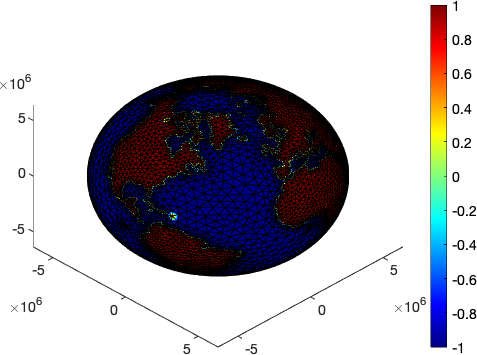
\includegraphics[scale=1.0]{/assets/img/using-issm/tutorials/greenland/Mesh.png}
	\end{center}
\end{figure}
%}}}
\subsection{Parameterization} %{{{
Call the \verb@setmask@ function with empty arguments, to denote that all ice is grounded. Then parameterize your mesh with file \verb@Greenland.par@. Next, set your flow equation to SSA for all. Read through the parameter file \verb@./Greenland.par@, which is similar to your PIG .par file, but for Greenland. Here, we are parameterizing a full continental domain, so all points along the domain boundary will be considered ice front. As a result, these boundaries do not need to be constrained, therefore the single point constraints variables will all be set to NaN.

Run step 2. This will save your parameterized model. Now, plot the new model thickness and velocity. For example:
\begin{verbatim}>> plotmodel(md,'data',md.geometry.thickness)
>> plotmodel(md,'data',md.initialization.vel,'caxis',[1e-1 1e4],'log',10)\end{verbatim}

\begin{figure}[H]
	\begin{center}
		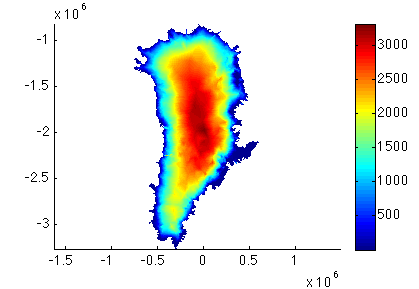
\includegraphics[scale=1.0]{/assets/img/using-issm/tutorials/greenland/Thickness.png}
	\end{center}
\end{figure}

\begin{figure}[H]
	\begin{center}
		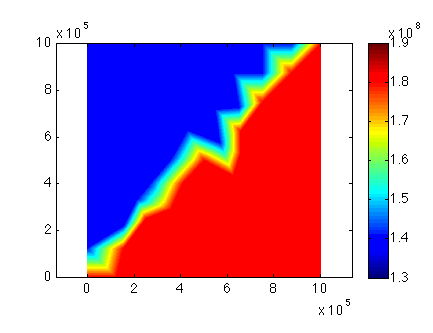
\includegraphics[scale=1.0]{/assets/img/using-issm/tutorials/greenland/Velocity.png}
	\end{center}
\end{figure}
%}}}
\subsection{Stress Balance} %{{{
Use control methods to inversely solve for Greenland FrictionCoefficient (Step 3, lines 44-81).

NOTE: Remember that \verb@md.inversion@ can be called for help!
\begin{itemize}
	\item Set three different cost functions
		\begin{itemize}
			\item Absolute value of surface velocity
			\item Log of surface velocity
			\item Drag coefficient gradient
		\end{itemize}
	\item Set cost functions coefficients to 350, 0.2, and\verb@ 2*10^-6@
	\item Set gradient scaling to 50
	\item Specify max inversion parameter = 200, min inversion parameter = 1
	\item Solve a 30-step Stress Balance model in 2D, SSA
	\item Copy result Friction Coefficient to model (\verb@md@) value
	\item Save your model
\end{itemize}

Review step 3 in the \verb@runme.m@ to verify that the parameters have been set properly. Run step 3 in the \verb@runme.m@ to perform the steps above.
%}}}
\subsection{Transient} %{{{
You are now ready to run a transient! In Step 4, we will simulate a simple constant warming trend over Greenland by forcing a temporal decrease in \verb@md.smb.mass_balance@.

\begin{figure}[H]
	\begin{center}
		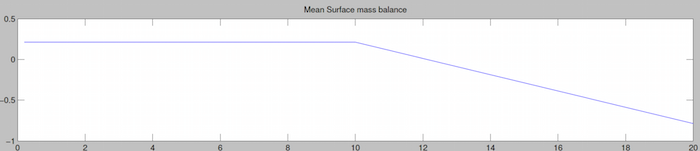
\includegraphics[scale=0.25]{/assets/img/using-issm/tutorials/greenland/TransientSMB.png}
	\end{center}
\end{figure}

Specify a transient forcing by adding a time value to the end (in the end+1 position) of the column of forcing variable values. For example, let SMB be the initial values of surface mass balance. To impose the forcing such that before time 10, surface mass balance is set to the column vector \verb@smb@, and after time 20, it is set to \verb@smb-1@ we use the following code:
\begin{itemize}
	\item \begin{verbatim}>> md.smb.mass_balance = [smb smb-1]
>> md.smb.mass_balance = [md.smb.mass_balance; [10 20]]\end{verbatim}
\end{itemize}

By default, ISSM will linearly interpolate surface mass balance between time 10 and time 20 in this example. Prior to first and after last imposed time, forcing values remain constant. In order to turn interpolation off (i.e. use a step function), you would set \verb@md.timestepping.interp_forcings=0@. If this values is set to 0, then your surface mass balance will change at the specified time, and will remain constant until a new value (column vector with time in the last row) is specified.

Steps to set up your transient:
\begin{itemize}
	\item Set control \verb@md.inversion.iscontrol@ back to 0
	\item Interpolate surface mass balance from SeaRISE dataset, converting from water to ice equivalent
	\item Impose SeaRISE surface mass balance for 10 years then linearly decrease to 1 m/yr by year 20
	\item Set time step to 0.2 and output frequency to 1 (every time step will be output in results)
	\item Ask your model to save IceVolume, TotalSmb, and SmbMassBalance transient output
	\item Solve a 20 year Transient in 2D, SSA
	\item Save your model
	\item Review lines 83-112 in \verb@runme.m@
\end{itemize}

In Step 5, we give you an example of how to plot the transient results (lines 114-145). To see how the transient results are stored in your model, type \verb@md.results.TransientSolution@.

Now, run steps 4 and 5 to launch your transient and plot results.
\begin{figure}[H]
	\begin{center}
		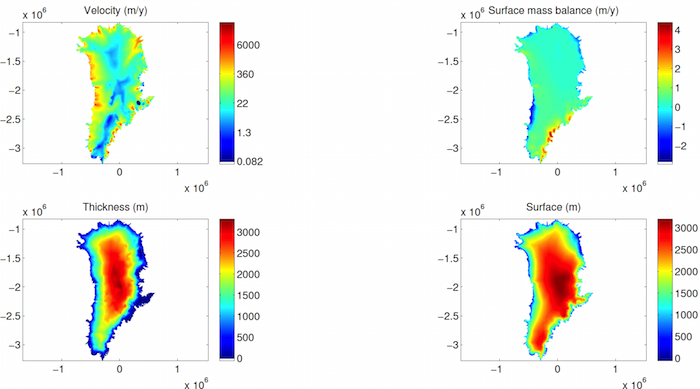
\includegraphics[scale=0.25]{/assets/img/using-issm/tutorials/greenland/ThicknessVelocity.png}
	\end{center}
\end{figure}

\begin{figure}[H]
	\begin{center}
		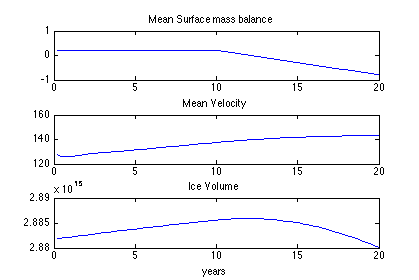
\includegraphics[scale=1.07]{/assets/img/using-issm/tutorials/greenland/Transient.png}
	\end{center}
\end{figure}
%}}}
\subsection{Exercise} %{{{
Now, let's run our transient with historical mass balance! Use Jason Box's surface mass balance (SMB) time series as forcing \citep{Box2013a,Box2013b,Box2013c}.\textsuperscript{1}

First, format the SMB provided. In Step 6 of the \verb@runme.m@ file, we extract the SMB timeseries from the NetCDF file, and create a timeseries plot (lines 147-175). Execute step 6. This will result in the figure below:
\begin{figure}[H]
	\begin{center}
		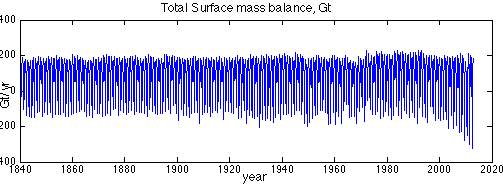
\includegraphics[scale=0.9]{/assets/img/using-issm/tutorials/greenland/HistoricalMassBalance.png}
	\end{center}
\end{figure}

In Step 7, we will relax the model towards equilibrium with the mean SMB forcing. An example of a 20 year relaxation to the time series mean is shown in \verb@runme.m@, step 7. Run step 7, which will assign the mean SMB to \verb@md.smb.mass_balance@ and run a transient model for 20 years, with a timestep of 0.2 years, saving the results every timestep. Step 7 will save the results in the Model "\verb@Greenland.HistoricTransient@."

To plot the relaxed version of the model that you just created, change step 5 to load the model "\verb@Greenland.HistoricTransient@" rather than "\verb@Greenland.Transient@," and run step 5 again.

\begin{figure}[H]
	\begin{center}
		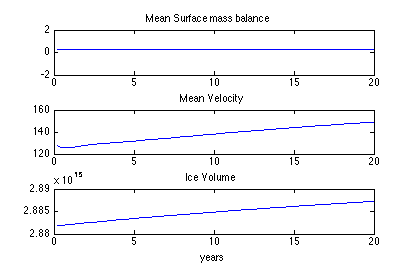
\includegraphics[scale=1.1]{/assets/img/using-issm/tutorials/greenland/Transient2.png}
	\end{center}
\end{figure}

To reach equilibrium, the model should run on the order of 3000 years. Since, 3000 years might take quite a long time to run on a personal computer, you may want to try running for 200 years instead.

To accomplish this extended relaxation, alter step 7 to run for the extended time period (200 years instead of 20 years). In the last line of this step, save your model as \verb@./Models/Greenland.HistoricTransient_200yr@ instead of \verb@./Models/Greenland.HistoricTransient@, to avoid overwriting the old model. Then, run step 7 again. This run of 200 years will take longer than your original 20 year run.

When you are done with step 7, complete step 8 on your own as an exercise. Fill in the required code to plot the results in step 8. Follow the comments, write the code to load the historic transient model, and create line plots of relaxation run (use Step 5 as a reference). Then, save surface mass balance by looping through 200 years (i.e. 1000 steps). Plot the surface mass balance time series in the first subplot. Title this plot "Mean Surface Mass Balance".

Next, save velocity by looping through 1000 steps. Plot velocity time series in a second subplot. Title this plot "Mean Velocity".

Lastly, save Ice Volume by looping through 1000 steps. Plot volume time series in a third subplot. Title this plot "Ice Volume" and add an x label of "years". The resulting plot should look like this:

\begin{figure}[H]
	\begin{center}
		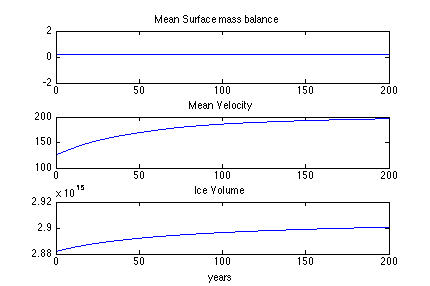
\includegraphics[scale=1.1]{/assets/img/using-issm/tutorials/greenland/200TimeSeries.png}
	\end{center}
\end{figure}

In Step 9, we will use the 200 year relaxed ice sheet as a starting condition for a historic transient run. To do so we need to save the 200 year resulting geometry and velocities into the model state. To load your past results see lines 254-259.

Next, we load the Box time series saved earlier in mat file, \verb@smbbox.mat@, and then (lines 261-300):
\begin{itemize}
	\item Interpolate every month of Box SMB onto the ISSM grid: insert a column for each month
	\item Add a final row indicating that the value should be set in the middle of each month
	\item Solve at a monthly time step and save monthly results
\end{itemize}

Run step 9, which will execute your historical transient forward simulation, monthly from 2003-2012.

Then, run step 10 to plot a time series of total surface mass balance, max velocity, and ice volume. See Lines 305-329.

\begin{figure}[H]
	\begin{center}
		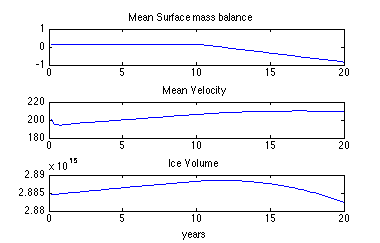
\includegraphics[scale=1.05]{/assets/img/using-issm/tutorials/greenland/MassVelocityVolume.png}
	\end{center}
\end{figure}

\subsection{Solution for step 7} %{{{
\begin{verbatim}if any(steps==7)
	disp('  Step 7: Historical Relaxation run');
	md = loadmodel('./Models/Greenland.Control_drag');

	load smbbox

	%convert mesh x,y into the Box projection
	[md.mesh.lat,md.mesh.long] = xy2ll(md.mesh.x,md.mesh.y,+1,39,71);
	[xi,yi]= ll2xy(md.mesh.lat,md.mesh.long,+1,45,70);

	%Interpolate and set surface mass balance
	index = BamgTriangulate(x1(:),y1(:));
	smb_mo = InterpFromMeshToMesh2d(index,x1(:),y1(:),smbmean(:),xi,yi);
	smb = smb_mo*12/1000*md.materials.rho_freshwater/md.materials.rho_ice;
	md.smb.mass_balance = [smb;1 ];

	%Set transient options, run for 20 years, saving every 5 timesteps
	md.timestepping.time_step=0.2;
	md.timestepping.final_time=200;
	md.settings.output_frequency=5;

	%Additional options
	md.inversion.iscontrol=0;
	md.transient.requested_outputs={'IceVolume','TotalSmb', ...
		'SmbMassBalance'};
	md.verbose=verbose('solution',true,'module',true);

	%Go solve
	md.cluster=generic('name',oshostname,'np',2);
	md=solve(md,'Transient');
	
	save ./Models/Greenland.HistoricTransient_200yr md;
end\end{verbatim}
%}}}

\subsection{Solution for step 8} %{{{
\begin{verbatim}if any(steps==8)
	%Load historic transient model
	md=loadmodel('./Models/Greenland.HistoricTransient_200yr');

	%Create Line Plots of relaxation run. Create a figure.
	figure;

	%Save surface mass balance, by looping through 200 years (1000 steps)
	%Note, the first output will always contain output from time step 1
	surfmb=[];
	for i=2:201;
		surfmb=[surfmb md.results.TransientSolution(i).SmbMassBalance];
	end

	%Plot surface mass balance time series in first subplot
	subplot(3,1,1);
	plot([1:200],mean(surfmb));

	%Title this plot Mean surface mass balance
	title('Mean Surface mass balance');

	%Save velocity by looping through 200 years
	vel=[];
	for i=2:201;
		vel=[vel md.results.TransientSolution(i).Vel];
	end

	%Plot velocity time series in second subplot
	subplot(3,1,2);
	plot([1:200],mean(vel));

	%Title this plot Mean Velocity
	title('Mean Velocity');

	%Save Ice Volume by looping through 200 years
	volume=[];
	for i=2:201;
		volume=[volume md.results.TransientSolution(i).IceVolume];
	end

	%Plot volume time series in third subplot
	subplot(3,1,3);
	plot([1:200],volume);

	%Title this plot Mean Velocity and add an x label of years
	title('Ice Volume');
	xlabel('years');
end\end{verbatim}
%}}}

\textsuperscript{1} \small{The year 1840-2012 Greenland near surface air temperature (T) and land ice SMB reconstruction after Box [2013] is calibrated to RACMO2 output \citep{Meijgaard2008,Ettema2009,Broeke2009,Angelen2011}. The calibration for T and SMB components is based on the 53 year overlap period 1960-2012. The calibration for snow accumulation rate is shorter because ice core data availability drops after 1999. Calibration is made using linear regression coefficients for 5 km grid cells that match the average of the reconstruction to RACMO2. The RACMO2 data are resampled and reprojected from the native 0.1 deg ($\sim$10 km) grid to a 5 km grid better resolving areas where sharp gradients occur, especially near the ice margin where mass fluxes are largest. Several refinements are made to the Box [2013] temperature (T) and SMB reconstruction. Multiple station records now contribute to the near surface air temperature for each given year, month and grid cell in the domain while in Box [2013], data from the single highest correlating station yielded the reconstructed value. The estimation of values is made for a domain that includes land, sea, and ice. Box [2013] reconstructed T over only ice. A physically-based meltwater retention scheme \citep{Pfeffer1990,Pfeffer1991} replaces the simpler approach used by Box [2013]. The RACMO2 data have a higher native resolution of 11 km as compared to the 24 km Polar MM5 data used by Box [2013] for air temperatures. The revised surface mass balance data end two years later in year 2012. The annual accumulation rates from ice cores are dispersed into a monthly temporal resolution by weighting the monthly fraction of the annual total for each grid cell in the domain evaluated using a 1960-2012 RACMO2 data.}
%}}}
\subsection{Additional Exercises} %{{{
\begin{itemize}
	\item Increase SMB instead of decrease over time
	\item Create an instantaneous step in SMB forcing at 10 years instead of a steady change over time
	\item Create a more advanced SMB forcing, like cyclic steps or a curve
	\item Force SMB to change only in certain areas of the ice sheet
	\item Add more melt in the ablation zone, but more snow in the upper elevations
	\item Force another field transiently (e.g. friction coefficient)
	\item Run the Box time series yearly or for a longer subset of time. This could take a while!
\end{itemize}
%}}}
